\section{Experimental Setup}
\label{sec:exp-setup}
All experiments were executed on a dedicated, isolated machine under controlled conditions to maximize measurement stability and reproducibility.

\textbf{Hardware and system environment.}
Experiments were performed on an Intel CPU (model: \texttt{i7-6700K}; with 16\,GB DDR4 RAM, running Pop!\_OS 22.04 (64 bit). To reduce measurement noise, we stabilized the environment as in Section \ref{sec:enviromental_Stab}. We loaded the \texttt{msr} kernel module to access Model-Specific Registers for RAPL readings.


\textbf{Software environment.}
All experiments used Python~3.12. Block extraction relied on the standard \texttt{ast} module and custom instrumentation utilities. All code, experiment scripts, and seed values for pseudo-random operations are archived and available in the artifact repository. We set a fixed random seed for all learning experiments to ensure reproducible train/test splits and model initializations.

\textbf{Dataset.}
The dataset was constructed from a larger corpus of Python programs\footnote{\url{https://huggingface.co/datasets/iamtarun/python_code_instructions_18k_alpaca}}. After parsing with \texttt{ast}, we extracted executable code blocks defined as function bodies, loop bodies (\texttt{for}, \texttt{while}), conditional bodies (\texttt{if}), exception handlers (\texttt{try/except}), and context manager blocks (\texttt{with}). We filtered out non-executable blocks as we need ground truth measurements. From \textbf{18,612} code files, we extract \textbf{14,000+} executable blocks, retaining \textbf{8,000+} that exceed 1 µs (measurable with N=1000). Each block was annotated with a set of \textbf{33 static features} comprising of AST derived features and standard code properties.

\textbf{Measurement protocol.}
Energy readings were taken from processor energy counters exposed via Intel RAPL through MSR access. Specifically, we read the \texttt{PACKAGE} domains using the MSR interface. All MSR reads were executed with root privileges and synchronized with our measurement control loop to avoid partial-window reads. 
Block execution times are typically in the microsecond range, while RAPL updates at millisecond granularity; to bridge this mismatch we used deterministic amplification and synchronization as follows:

% \begin{enumerate}

%   \item \textbf{Amplification:} each target block was executed in a tight loop of $N$ consecutive iterations (we used $N=1000$), and the total energy measured across the loop was divided by $N$ to yield a per-iteration estimate. The value of $N$ was chosen to produce a signal that is reliably captured by RAPL while keeping total runtime reasonable.
%   \item \textbf{Synchronization and padding:} before starting an amplification loop we ensured the RAPL counters had updated (fresh window) and, after the loop, appended a calibrated empty loop (padding) whose energy cost was measured separately and subtracted from the aggregate reading to compensate for loop/overhead energy.
%   \item \textbf{Repetitions and outlier-handling:} Each amplified measurement was repeated $m=10$ times; we discarded statistical outliers using interquartile-range (IQR) filtering and used the mean of the remaining trials as the final block energy estimate. The outliers occured due to randomly occuring system flareups that affect energy usage.
%   \item \textbf{Environment stabilization:} between block measurements we allowed a short cool-down period and ensured background system activity remained minimal. The CPU governor remained set to \texttt{performance} throughout; Turbo Boost and other dynamic frequency controls were disabled to avoid transient frequency-induced variability.
% \end{enumerate}

% \paragraph{Baseline validation.}
% To validate aggregated block-level energy, we compared summed PowerLens measurements against coarse-grained program-level energy reported by PyRAPL (or an equivalent RAPL wrapper). The aggregated block sums were consistent with PyRAPL measurements across block categories (see Figure~\ref{fig:powerlens-pyrapl}).

\textbf{Evaluation protocol and statistical analysis.}
We evaluated both regression and classification formulations. Regression performance metrics include R² (variance explained), RMSE (root mean squared error), MAE (mean absolute error), and MAPE (mean absolute percentage error) \cite{Botchkarev2018PerformanceM}\cite{Chicco2021TheCO}. For classification (energy-tier prediction), we report accuracy (correct predictions), precision (positive prediction accuracy), recall (true positive coverage), F1-score (harmonic mean of precision and recall), and confusion matrices \cite{SOKOLOVA2009427}. All reported results include mean and standard deviation across folds.


% \begin{figure}[t]
%   \centering
%   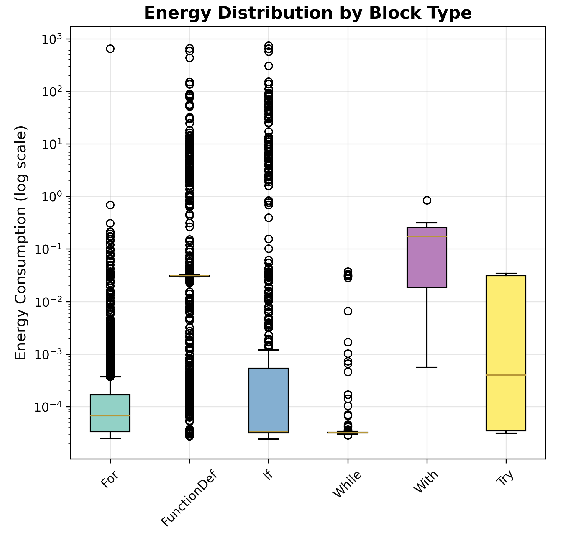
\includegraphics[width=0.9\linewidth]{figures/energy_distribution_by_block_type.png}
%   \caption{Energy consumption distribution across different block types.}
%   \label{fig:energy-distribution-block-type}
% \end{figure}
